\documentclass{beamer}\usepackage[]{graphicx}\usepackage[]{color}
% maxwidth is the original width if it is less than linewidth
% otherwise use linewidth (to make sure the graphics do not exceed the margin)
\makeatletter
\def\maxwidth{ %
  \ifdim\Gin@nat@width>\linewidth
    \linewidth
  \else
    \Gin@nat@width
  \fi
}
\makeatother

\definecolor{fgcolor}{rgb}{0.345, 0.345, 0.345}
\newcommand{\hlnum}[1]{\textcolor[rgb]{0.686,0.059,0.569}{#1}}%
\newcommand{\hlstr}[1]{\textcolor[rgb]{0.192,0.494,0.8}{#1}}%
\newcommand{\hlcom}[1]{\textcolor[rgb]{0.678,0.584,0.686}{\textit{#1}}}%
\newcommand{\hlopt}[1]{\textcolor[rgb]{0,0,0}{#1}}%
\newcommand{\hlstd}[1]{\textcolor[rgb]{0.345,0.345,0.345}{#1}}%
\newcommand{\hlkwa}[1]{\textcolor[rgb]{0.161,0.373,0.58}{\textbf{#1}}}%
\newcommand{\hlkwb}[1]{\textcolor[rgb]{0.69,0.353,0.396}{#1}}%
\newcommand{\hlkwc}[1]{\textcolor[rgb]{0.333,0.667,0.333}{#1}}%
\newcommand{\hlkwd}[1]{\textcolor[rgb]{0.737,0.353,0.396}{\textbf{#1}}}%
\let\hlipl\hlkwb

\usepackage{framed}
\makeatletter
\newenvironment{kframe}{%
 \def\at@end@of@kframe{}%
 \ifinner\ifhmode%
  \def\at@end@of@kframe{\end{minipage}}%
  \begin{minipage}{\columnwidth}%
 \fi\fi%
 \def\FrameCommand##1{\hskip\@totalleftmargin \hskip-\fboxsep
 \colorbox{shadecolor}{##1}\hskip-\fboxsep
     % There is no \\@totalrightmargin, so:
     \hskip-\linewidth \hskip-\@totalleftmargin \hskip\columnwidth}%
 \MakeFramed {\advance\hsize-\width
   \@totalleftmargin\z@ \linewidth\hsize
   \@setminipage}}%
 {\par\unskip\endMakeFramed%
 \at@end@of@kframe}
\makeatother

\definecolor{shadecolor}{rgb}{.97, .97, .97}
\definecolor{messagecolor}{rgb}{0, 0, 0}
\definecolor{warningcolor}{rgb}{1, 0, 1}
\definecolor{errorcolor}{rgb}{1, 0, 0}
\newenvironment{knitrout}{}{} % an empty environment to be redefined in TeX

\usepackage{alltt}

\usepackage[backend=bibtex, sorting=none, style=chicago-authordate]{biblatex}
\addbibresource{scRNA.bib}
\renewcommand*{\bibfont}{\scriptsize}

\mode<presentation>
{
 \usetheme{AnnArbor}
 \usecolortheme{seahorse}
}
\setbeamertemplate{navigation symbols}{}
\usepackage[english]{babel}
\usepackage{times}
\usepackage[T1]{fontenc}
%\usepackage[applemac]{inputenc}
\usepackage{amsmath}
%\usepackage{tikz}
\usepackage[font=footnotesize,labelfont=bf]{caption} 
\usepackage{mwe,tikz}
\usepackage[percent]{overpic}
\usepackage{amssymb}

\setbeamerfont{caption}{size=\scriptsize}
\setbeamertemplate{caption}{\raggedright\insertcaption\par}
\usepackage{hyperref}  
\hypersetup{colorlinks=true,allcolors=blue}

\title[scRNA-seq DE]{scRNA-seq}
\subtitle{Differential expression analyses}
%\author[Olga]{Olga Dethlefsen}
\author[Olga]{Olga Dethlefsen\\{\scriptsize olga.dethlefsen@nbis.se}}
\institute[NBIS]{NBIS, National Bioinformatics Infrastructure Sweden\\}
\date[February 2019]{February 2019}

\logo{%
  
\includegraphics[height=1cm,keepaspectratio]{Images/SciLifeLab-logo.jpg}%
  \hspace{\dimexpr\paperwidth-5cm-5pt}%
  
\includegraphics[height=1cm,keepaspectratio]{Images/nbislogo-orange.png}%
}
\usepackage{textpos}
\IfFileExists{upquote.sty}{\usepackage{upquote}}{}
\begin{document}

% Title page
\begin{frame}
\titlepage
\end{frame}

\logo{}

% Outline
\section{Outline}
\begin{frame}
\begin{block}{Outline}
\begin{itemize}  \pause
  \item Introduction: what is so special about scRNA-seq DE? \pause
  \item Common methods: what is out there? \pause
  \item Performance: how do we know what is best? \pause
  \item Practicalities: what to do in real life? \pause
  \item Summary: what to remember from this hour? 
  %\item DE tutorial
 \end{itemize}
\end{block}
\end{frame}

\section{Introduction}
\begin{frame}
\begin{center}
\insertsection
\end{center}
\end{frame}

% Intro: defying differential expression (Menti)
\begin{frame}
\begin{center}
What does "differential expression" mean to you?
\begin{figure}
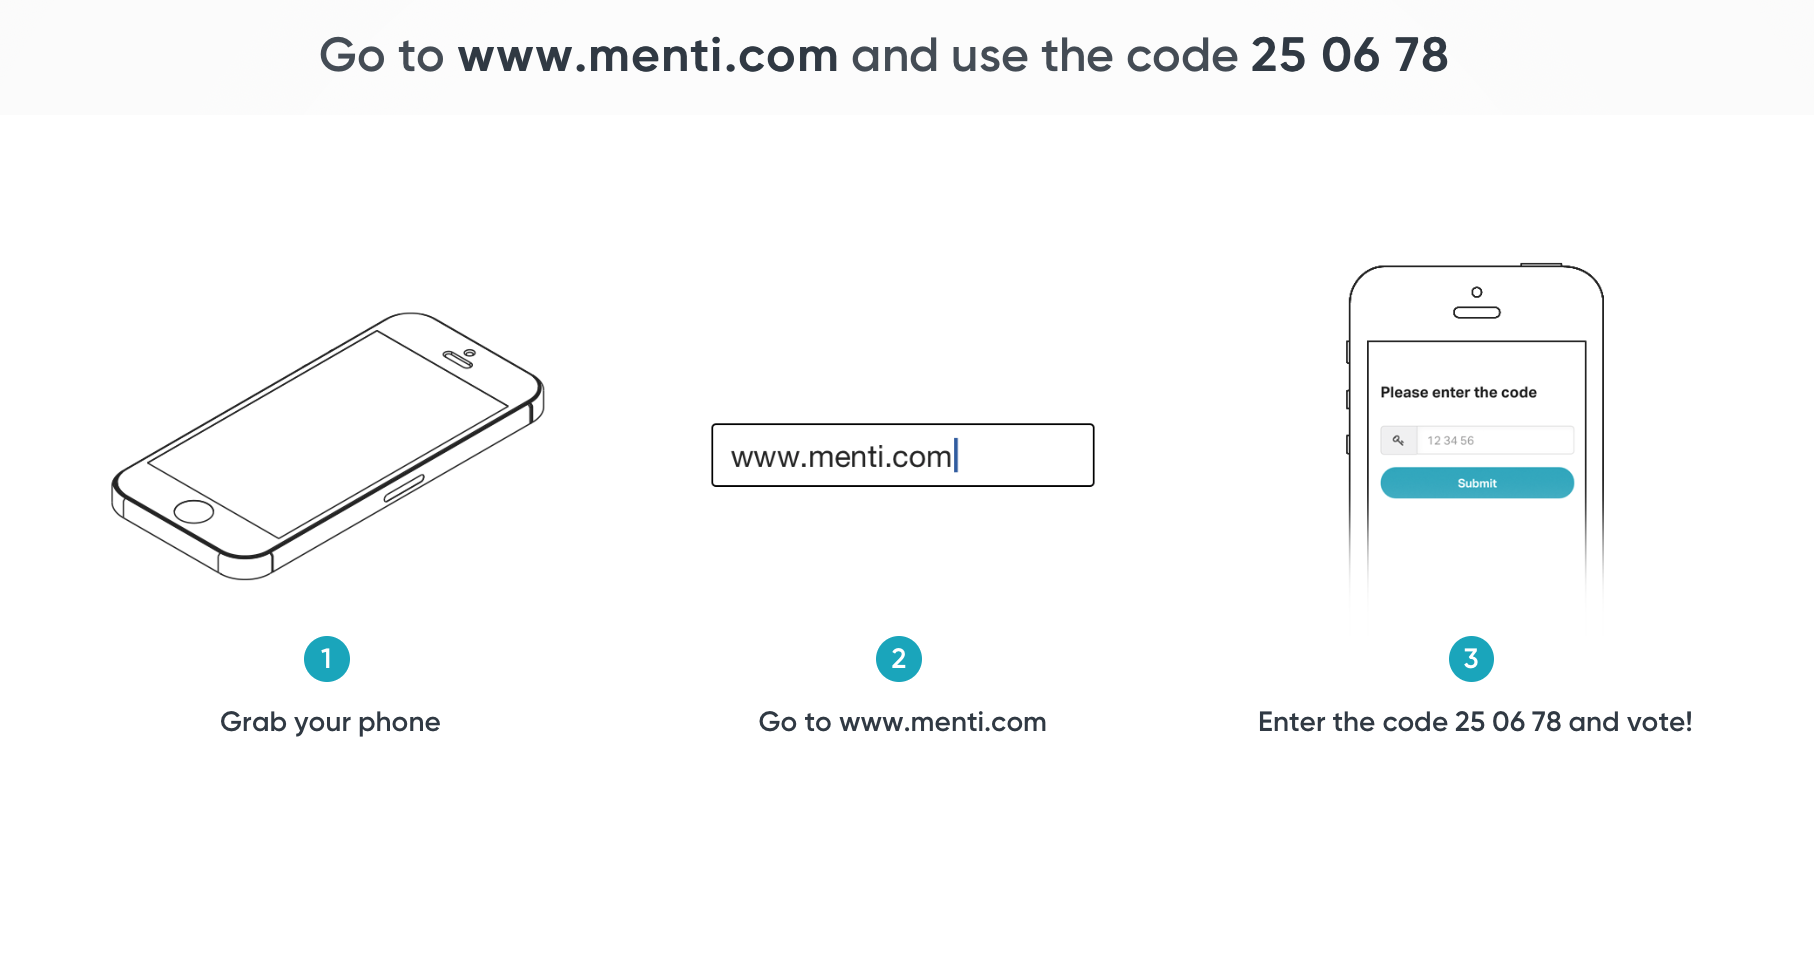
\includegraphics[width=12cm]{Images/menti.png}
\end{figure}
\href{https://www.menti.com}{https://www.menti.com}
\end{center}
\end{frame}

% Intro: Overview figure DE-01
\begin{frame}
\begin{center}
\begin{figure}
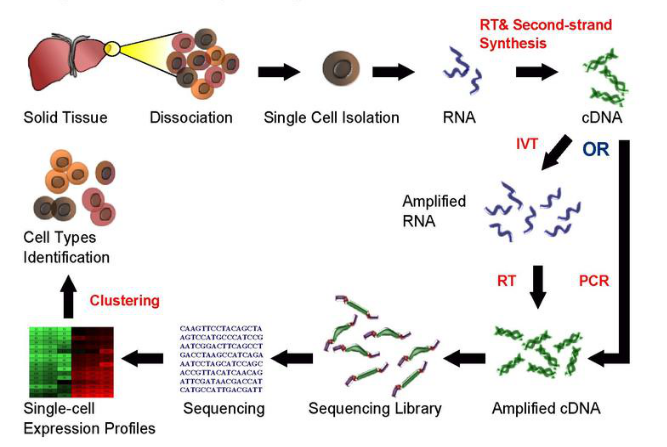
\includegraphics[width=10cm]{Images/DE-overview-01.png}
\caption{Figure: Simplified scRNA-seq workflow [adapted from Wikipedia]}
\end{figure}
\end{center}
\end{frame}

% Intro: Overview figure DE-02
\begin{frame}
\begin{center}
\begin{figure}
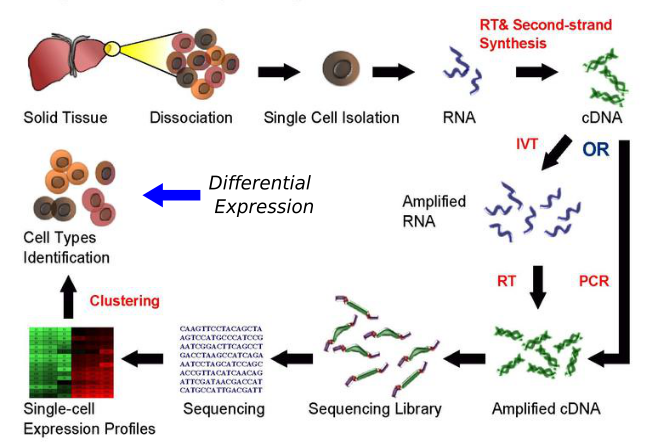
\includegraphics[width=10cm]{Images/DE-overview-02.png}
\caption{Figure: Simplified scRNA-seq workflow [adapted from Wikipedia]}
\end{figure}
\end{center}
\end{frame}

% Intro: defying differential expression
\begin{frame}
\begin{columns}

\column{0.4\textwidth}
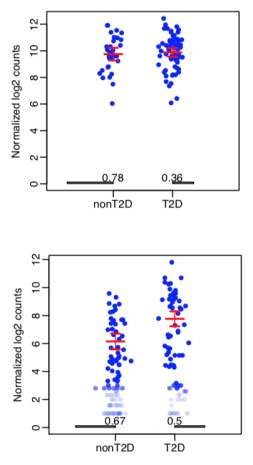
\includegraphics[width=4.5cm, height=7.5cm]{Images/Wu-2017-01.png}
\captionof{figure}{adapted from \cite{Wu2017}}

\column{0.6\textwidth}
Differential expression means
\scriptsize
\begin{itemize}
  \item taking read count data \&
  \item performing statistical analysis to discover quantitative changes in expression levels between experimental groups
  \item i.e. to decide whether, for a given gene, an observed difference in read counts is significant (greater than what would be expected just due to natural random variation)
 \end{itemize} \pause
\vspace{0.5cm}
\normalsize 
Differential expression is an old "problem"
\scriptsize
\begin{itemize}
  \item known from bulk RNA-seq and microarray studies
  \item in fact building on one of the most common statistical problems, i.e comparing groups for statistical differences
 \end{itemize}

\end{columns}
\end{frame}

% Intro: Question
\begin{frame}
\begin{center}
\colorbox{blue!10}{Differential expression is an old problem.}
\colorbox{blue!10}{So what is all the commotion about?}
%\vspace{0.2cm}
\end{center}
\begin{center}
\href{https://www.menti.com}{https://www.menti.com} \& 25 06 78 \pause
\end{center}
\vspace{0.5cm}
\begin{block}{scRNA-seq: special characteristics}
\begin{itemize}
 \item high noise levels (technical and biological factors)
  \item low library sizes
  \item low amount of available mRNAs results in amplification biases and "dropout events"
  \item 3' bias, partial coverage and uneven depth (technical)
  \item stochastic nature of transcription (biological)
  \item multimodality in gene expression; presence of multiple possible cell states within a cell population (biological)
 \end{itemize}
\end{block}
\end{frame}

\begin{frame}
\begin{center}
\begin{figure}
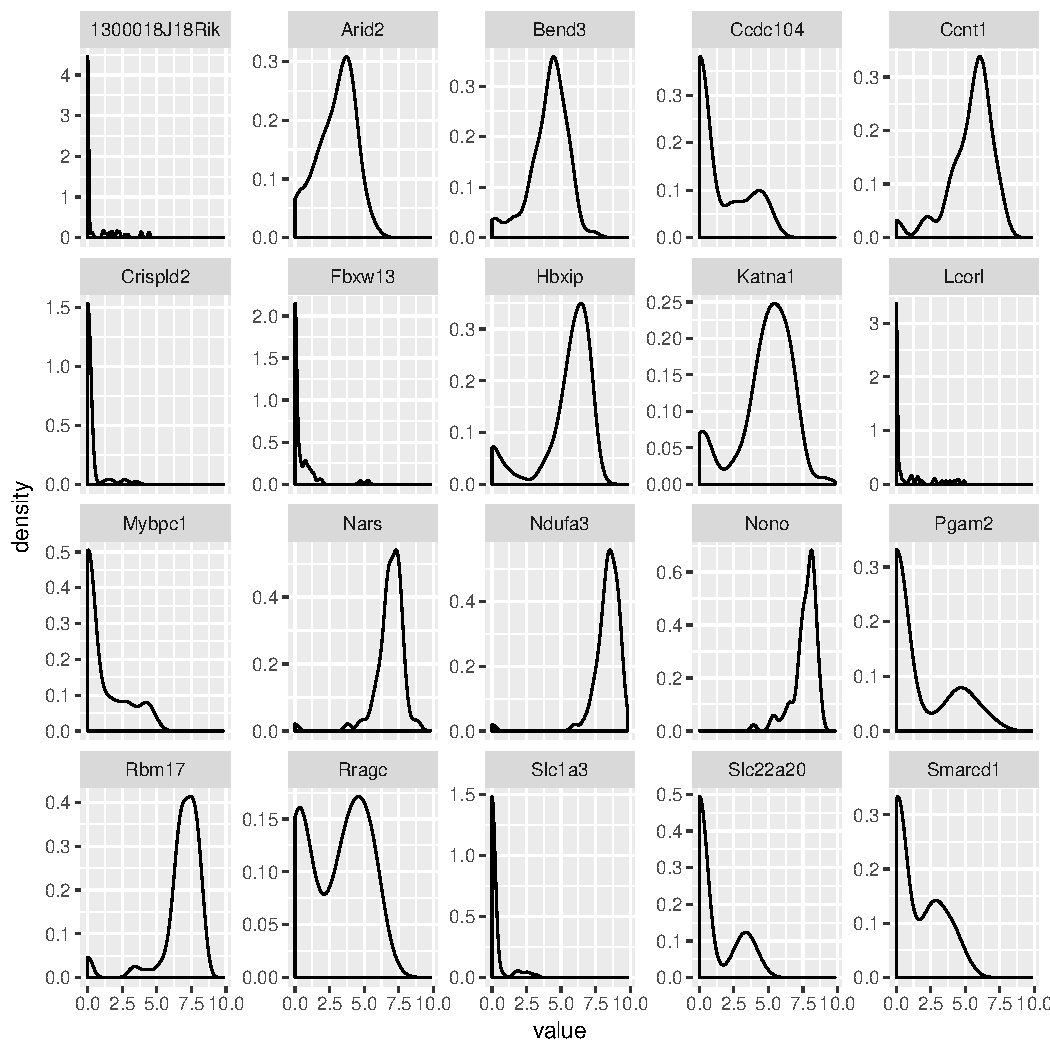
\includegraphics[width=10cm, height=7.5cm]{Images/ZeroInflated-biomodal.pdf}
\caption{Based on tutorial data}
\end{figure}
\end{center}
\end{frame}


\section{Common methods}
% Section slide
\begin{frame}
\begin{center}
\insertsection
\end{center}
\end{frame}

% CM: Triangle
\begin{frame}
\begin{center}
\begin{figure}
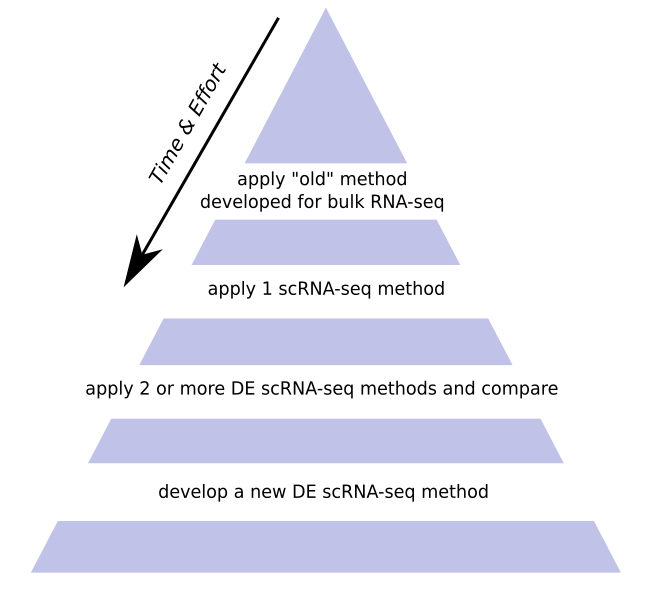
\includegraphics[width=10cm]{Images/solutionTriangle.png}
\caption{Simplified scRNA-seq workflow [adopted from \href{http://hemberg-lab.github.io/]}{http://hemberg-lab.github.io/}}
\end{figure}
\end{center}
\end{frame}

% CM: Name methods: non-parametric
\begin{frame} %\pause
\begin{block}{Generic non-parametric methods}
\begin{itemize}
\small
  \item e.g. Wilcoxon rank-sum test, Kruskal-Wallis, Kolmogorov-Smirnov test
  \item non-parametric tests generally convert observed expression values to ranks \& test whether the distribution of ranks for one group are signficantly different from the distribution of ranks for the other group
  \item some non-parametric methods fail in the presence of a large number of tied values, such as the case for dropouts (zeros) in single-cell RNA-seq expression data
  \item if the conditions for a parametric test hold, then it will typically be more powerful than a non-parametric test.
\end{itemize}
\end{block}
\end{frame}


% CM: Name methods: bulk RNA-seqq
\begin{frame} %\pause
\begin{block}{developed for bulk RNA-seq}
\begin{itemize}
\small 
  \item e.g. edgeR, DE-seq2
  \item compare estimates of mean-expression (sample size)
  \item based on negative binomial distribution
  \item can be assessed by datasets where RNA-seq data has beeen validated by RT-qPCR
\end{itemize}
\end{block}
\end{frame}

% CM: Name methods: scRNA-seq
\begin{frame} %\pause
\begin{block}{developed for scRNA-seq}
\begin{itemize}
\small
  \item e.g. MAST, SCDE, Monocle, Pagoda, D$^3$E etc. 
  \item large number of samples (i.e. cells) for each group we are comparing in single-cell experiments. Thus we can take advantage of the whole distribution of expression values in each group to identify differences between groups 
  \item we usually do not have a defined set of experimental conditions; instead we try to  identify the cell groups by using an unsupervised clustering approach.
 \end{itemize}
\end{block}
\end{frame}

% CM: Miao Table 1
\begin{frame}
\begin{center}
\begin{figure}
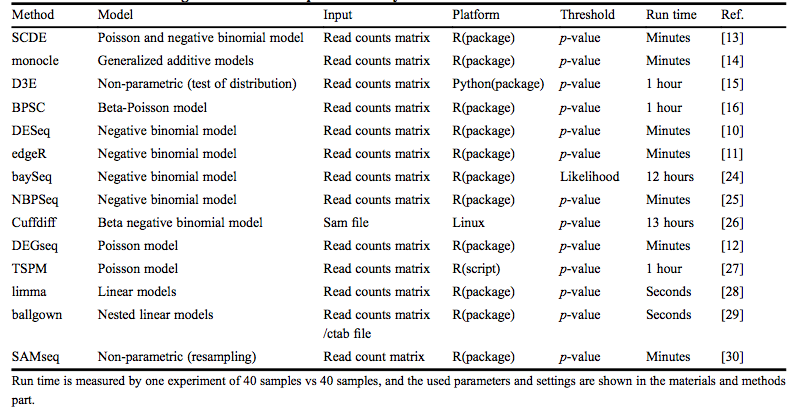
\includegraphics[width=10cm]{Images/MiaoTable1.png}
\caption{\cite{Miao2016}}
\end{figure}
\end{center}
\end{frame}

% CM: Robinson Table 2
\begin{frame}
\begin{center}
\begin{figure}
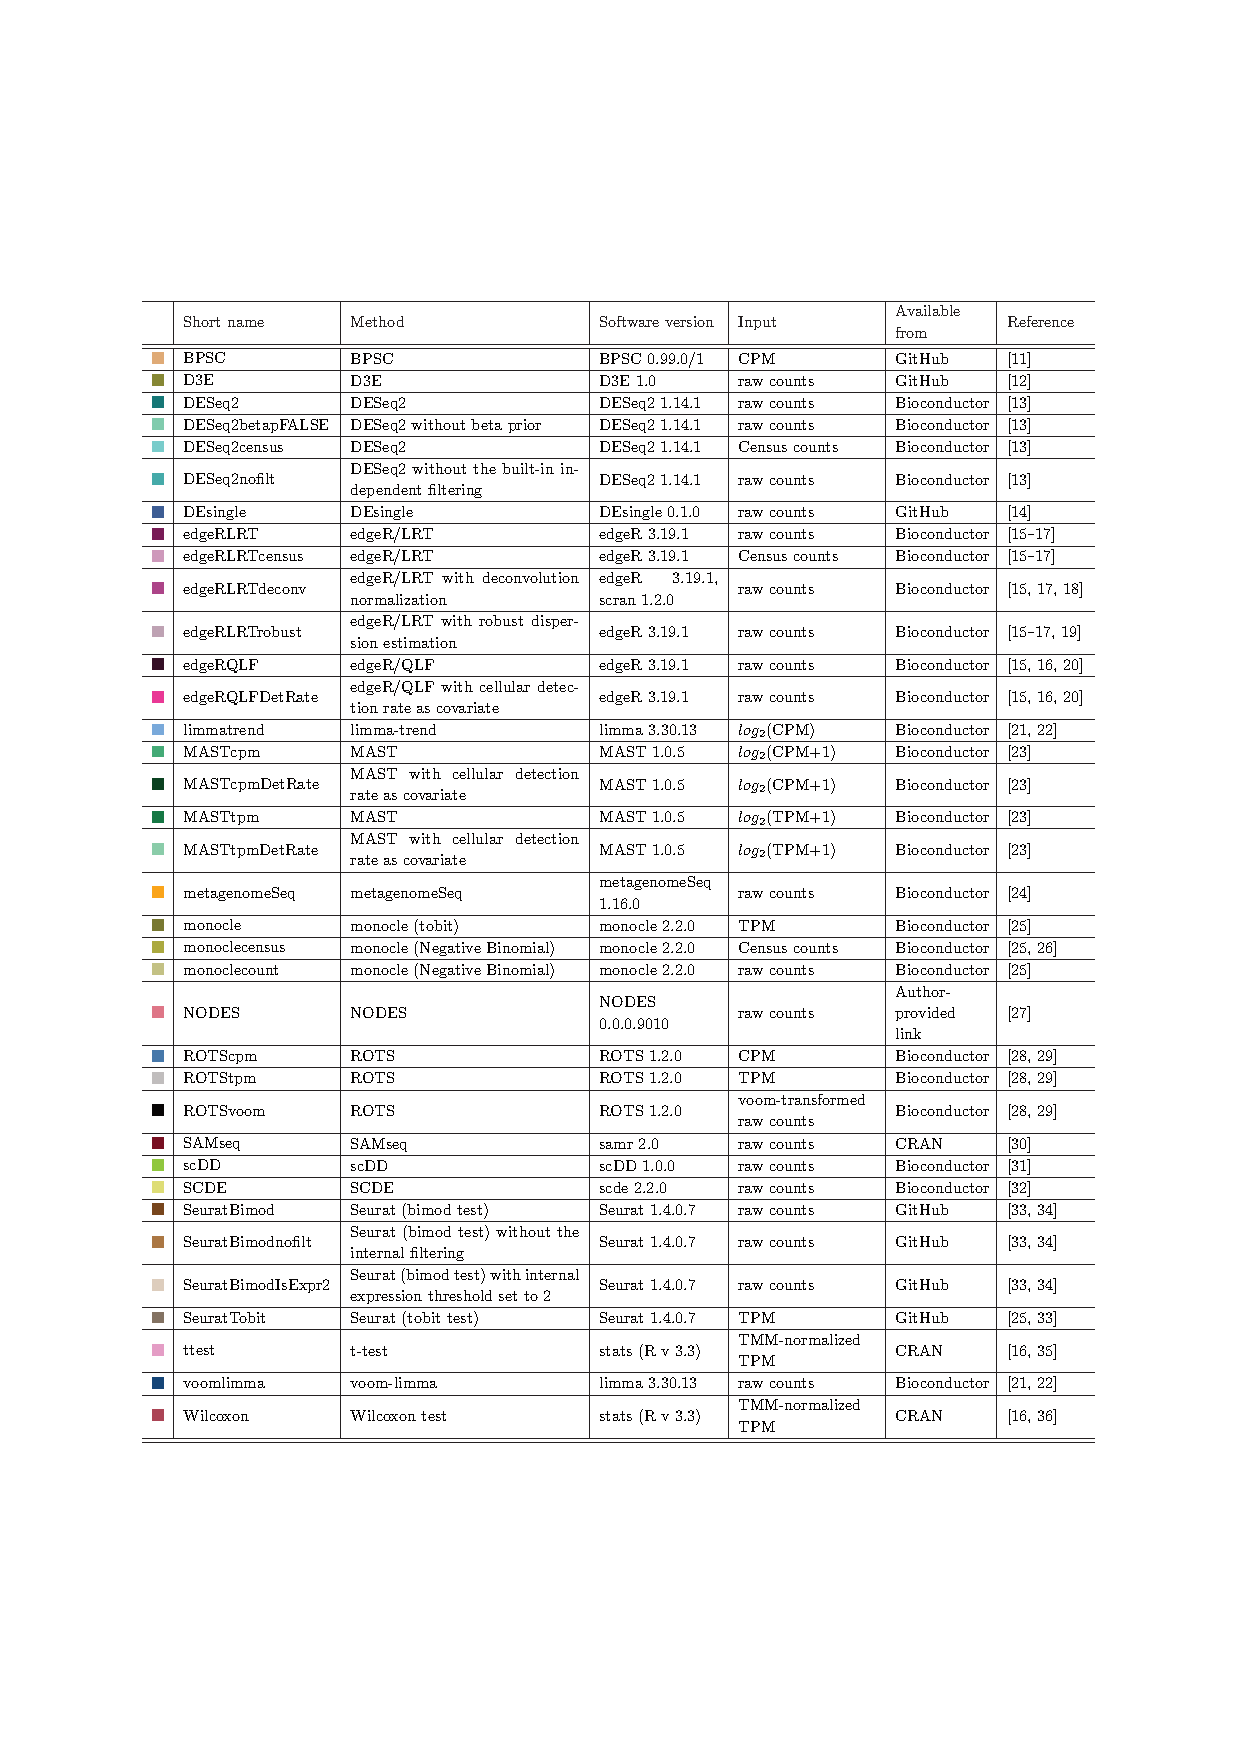
\includegraphics[trim={0 5cm 0 5cm}, clip, height=7.5cm]{Images/Robinson-2018.pdf}
\caption{\cite{Soneson2018}}
\end{figure}
\end{center}
\end{frame}

\subsection{More detailed examples}
% Section slide
\begin{frame}
\begin{center}
\insertsubsection
\end{center}
\end{frame}

% CM: MAST
\begin{frame}
%\frametitle{MAST}
\begin{block}{MAST}
\vspace{0.5cm}
\scriptsize
\begin{itemize}
  \item uses \underline{generalized linear hurdle model}
  \item designed to account for stochastic dropouts and bimodal expression distribution in which expression is either strongly non-zero or non-detectable
  \item The rate of expression \textbf{\textit{Z}}, and the level of expression \textbf{\textit{Y}}, are modeled for each gene \textbf{\textit{g}}, indicating whether gene \textbf{\textit{g}} is expressed in cell \textbf{\textit{i}} (i.e., $Z_{ig}=0$ if $y_{ig}=0$ and $z_{ig}=1$ if $y_{ig}>0$)
  \item A \underline{logistic regression model} for the discrete variable \textbf{\textit{Z}} and a \underline{Gaussian linear model} for the continuous variable (Y|Z=1):
   \end{itemize}
   \begin{center}
    $logit (P_r(Z_{ig}=1))=X_i\beta_g^D$ \newline
    $P_r(Y_{ig}=Y|Z_{ig}=1)=N(X_i\beta_g^C,\sigma_g^2)$, where $X_i$ is a design matrix
\end{center}
\begin{itemize}
\item Model parameters are \underline{fitted} using an empirical Bayesian framework
\item Allows for a joint estimate of nuisance and treatment effects
\item DE is determined using \underline{the likelihood ratio test}
\end{itemize}
\end{block}
\end{frame}

% % CM: SCDE
% \begin{frame}
% \begin{block}{SCDE}
% \vspace{0.5cm}
% \scriptsize
% \begin{itemize}
%   \item \underline{models} the read counts for each gene using a mixture of a NB, negative binomial, and a Poisson distribution
%   \item \underline{NB distribution} models the transcripts that are amplified and detected
%   \item \underline{Poisson distribution} models the unobserved or background-level signal of transcripts that are not amplified (e.g. dropout events)
%   \item subset of robust genes is used to fit, via \underline{EM} algorithm, the parameters to the mixture of models
%   \item For DE, the posterior probability that the gene shows a fold expression difference between two conditions is computed using a \underline{Bayesian approach}
% \end{itemize}
% \end{block}
% \end{frame}
% 
% % CM: Monocole
% \begin{frame}
% \begin{block}{Monocole}
% \vspace{0.5cm}
% \scriptsize
% \begin{itemize}
% \item Originally designed for ordering cells by progress through differentiation stages (pseudo-time)
% \item The mean expression level of each gene is \underline{modeled with a GAM}, generalized additive model, which relates one or more predictor variables to a response variable as
% \end{itemize}
%    \begin{center}
%     $g(E(Y))=\beta_0+f_1(x_1)+f_2(x_2)+...+f_m(x_m)$ where Y is a specific gene expression level, $x_i$ are predictor variables, g is a link function, typically log function, and $f_i$ are non-parametric functions (e.g. cubic splines)
%   \end{center}
% \begin{itemize}
% \item The observable expression level Y is then modeled using GAM,
% \end{itemize}
% $E(Y)=s(\varphi_t(b_x, s_i))+\epsilon$ where $\varphi_t(b_x, s_i)$ is the assigned pseudo-time of a cell and $s$ is a cubic smoothing function with three degrees of freedom. The error term $\epsilon$ is normally distributed with a mean of zero
% \begin{itemize}
% \item The DE test is performed using an \underline{approx. $\chi^2$ likelihood ratio test}
% \end{itemize}
% \end{block}
% \end{frame}

% CM: Let's stop for a minute
\begin{frame}
%\frametitle{SCDE}
Let's stop for a minute...
\begin{center}
\begin{figure}

\includegraphics[width=5cm]{Images/frustration.png}
%\caption{Simplified scRNA-seq workflow [adopted from \href{http://hemberg-lab.github.io/]}{http://hemberg-lab.github.io/}}
\end{figure}
\end{center}
\end{frame}


% CM: The key: figure and equation
\begin{frame}
\begin{block}{The key}
\begin{center}
\begin{figure}
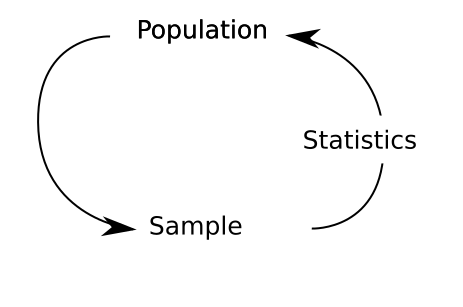
\includegraphics[width=5cm]{Images/stats.png}
\end{figure}
$Outcome_i=(Model_i)+error_i$
\end{center}
\begin{itemize}
\footnotesize
\item we collect data on a \underline{\textit{sample}} from a much larger \underline{\textit{population}}
\item \underline{\textit{statistics}} lets us to make inferences about the population from which sample was derived
\item we try to predict the outcome given a model fitted to the data
\end{itemize}
\end{block}
\end{frame}

% CM: The key: t-test example
\begin{frame}
%\frametitle{The key}
\begin{block}{The key}
\begin{flushright}
$t=\frac{x_1-x_2}{s_p\sqrt{\frac{1}{n_1}+\frac{1}{n_2}}}$
\end{flushright}
\begin{knitrout}
\definecolor{shadecolor}{rgb}{0.969, 0.969, 0.969}\color{fgcolor}
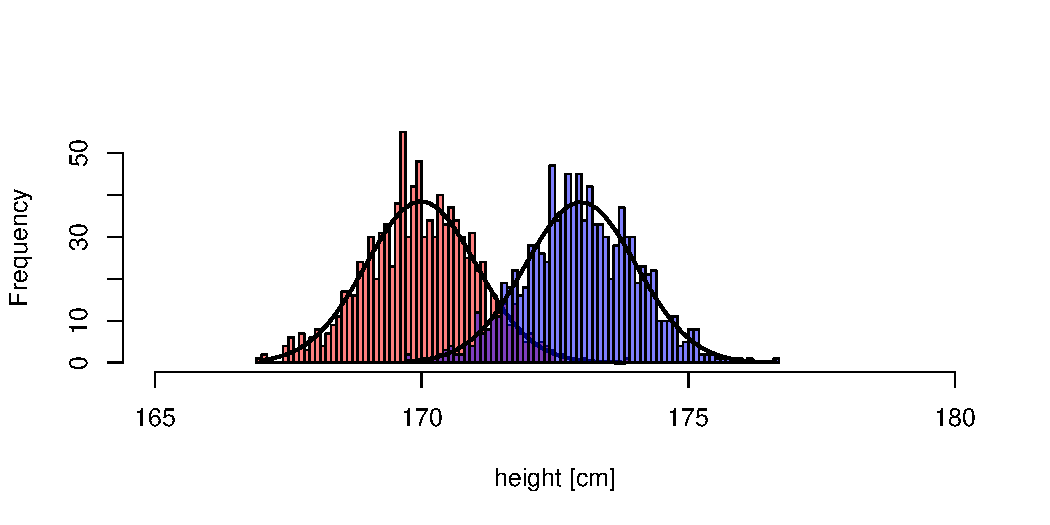
\includegraphics[width=\maxwidth]{figure/ttest-1} 

\end{knitrout}
\end{block}
\end{frame}


% CM: The most important equation
\begin{frame}
%\frametitle{The key}
\begin{block}{Generic recipe}
\begin{itemize}
\item model data e.g. gene expression
\item fit model to the data and/or data to the model
\item estimate model parameters
\item use model for prediction and/or inference
\end{itemize}
\end{block}
% \begin{block}{Implications}
% \begin{itemize}
% \item the better model fits to the data the better statistics
% \end{itemize}
% \end{block}
\end{frame}


% CM: The key implications
\begin{frame}
\begin{block}{Generic recipe}
\begin{itemize}
\item model e.g. gene expression with random error
\item fit model to the data and/or data to the model, estimate model parameters
\item use model for prediction and/or inference
\end{itemize}
\end{block}
\vspace{0.5cm}

\setbeamercolor{block title}{bg=red!10,fg=black}
\setbeamercolor{block body}{use=structure,fg=white,bg=red!30}
\begin{block}{Important implication}
the better model \href{http://www.itl.nist.gov/div898/handbook/pmd/section4/pmd44.htm}{fits} to the data the better statistics
\end{block}
\end{frame}


% CM: Distributions: negative binomial
\begin{frame}
\begin{block}{Common distributions}
\begin{knitrout}
\definecolor{shadecolor}{rgb}{0.969, 0.969, 0.969}\color{fgcolor}
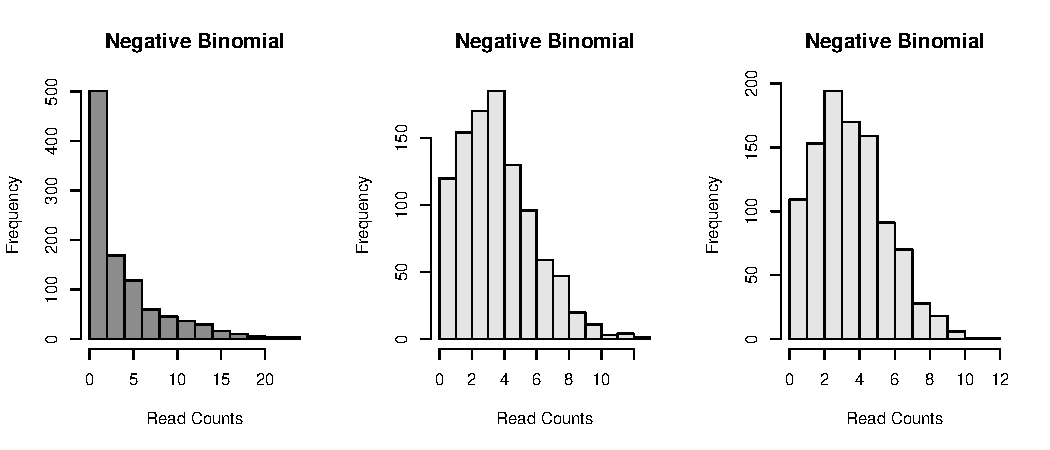
\includegraphics[width=\maxwidth]{figure/dist-NB-1} 

\end{knitrout}
\tiny
$$NeBi(\mu, \delta^2)$$
$$\mu=mu$$
$$\delta^2=mu+mu^2/size$$

\textit{mu}: mean expression, \textit{size}: and the dispersion, which is inversely related to the variance. NB fits bulk RNA-seq data very well and it is used for most statistical methods designed for such data. In addition, it has been show to fit the distribution of molecule counts obtained from data tagged by unique molecular identifiers (UMIs) quite well (Grun et al. 2014, Islam et al. 2011).

\end{block}
\end{frame}

% CM: Distributions: zero inflated NB
\begin{frame}
\begin{block}{Common distributions} % zero inflated model
\begin{knitrout}
\definecolor{shadecolor}{rgb}{0.969, 0.969, 0.969}\color{fgcolor}
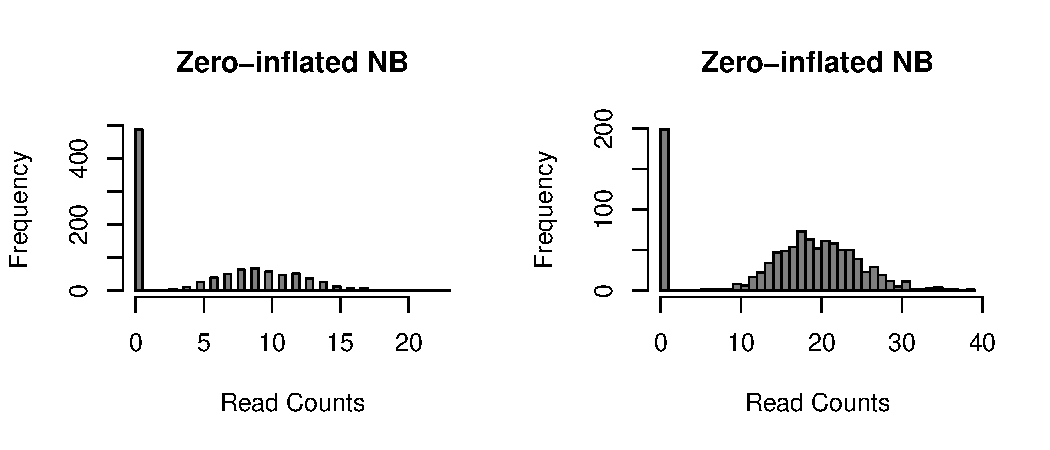
\includegraphics[width=\maxwidth]{figure/dist-zero-inlated-NB-1} 

\end{knitrout}

\tiny
$$NeBi(\mu, \delta^2)$$
$$\mu=mu*(1-d)$$
$$\delta^2=\mu*(1-d)*(1+d*\mu+\mu/size)$$

\textit{d}, dropout rate. The dropout rate of a gene is strongly correlated with the mean expression of the gene. Different zero-inflated negative binomial models use different relationships between \textit{mu} and \textit{d} and some may fit \textit{mu} and \textit{d} to the expression of each gene independently. Implemented in MAST, SCDE. 
\end{block}
\end{frame}

% CM: Distributions
\begin{frame}
\begin{block}{Common distributions} % Poisson
\begin{knitrout}
\definecolor{shadecolor}{rgb}{0.969, 0.969, 0.969}\color{fgcolor}
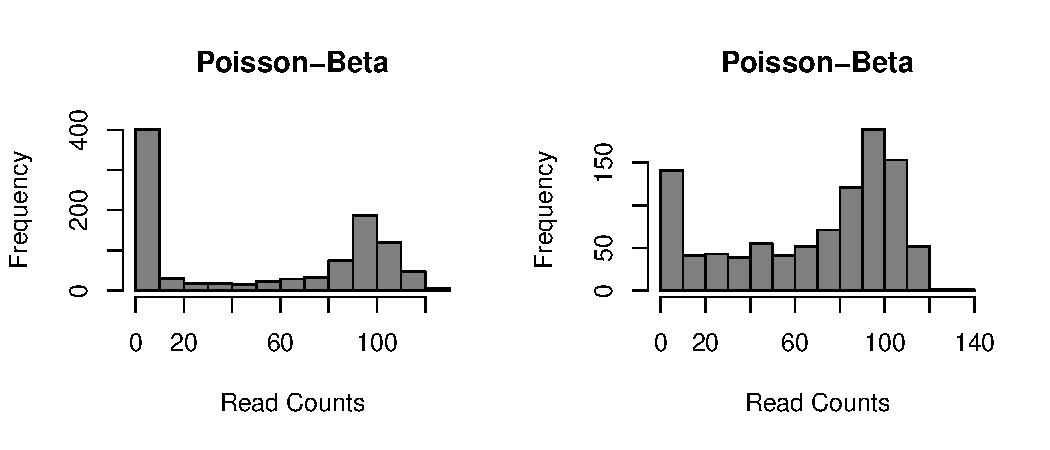
\includegraphics[width=\maxwidth]{figure/dist-poisson-beta-1} 

\end{knitrout}

\tiny
$$\mu=g*a/(a+b)$$
$$\delta^2=g^2*a*b/((a+b+1)*(a+b)^2)$$
% $$Poi(\lambda)$$
% $$\lambda = 1$$
% $$\lambda = 4$$

\textit{a}: the rate of activation of transcription; \textit{b} the rate of inhibition of transcription; and \textit{g} the rate of transcript production while transcription is active at the locus. Differential expression methods may test each of the parameters for differences across groups or only one (often \textit{g}). Implemented in BPSC.

May be further expanded to explicitly account for other sources of gene expression differences such as batch-effect or library depth depending on the particular DE algorithm. 
\end{block}
\end{frame}

\begin{knitrout}
\definecolor{shadecolor}{rgb}{0.969, 0.969, 0.969}\color{fgcolor}\begin{kframe}
\begin{alltt}
\hlkwd{graphics.off}\hlstd{()}
\hlkwd{par}\hlstd{(}\hlkwc{mfrow}\hlstd{=}\hlkwd{c}\hlstd{(}\hlnum{1}\hlstd{,}\hlnum{3}\hlstd{))}
\hlkwd{hist}\hlstd{(}\hlkwd{rpois}\hlstd{(}\hlnum{1009}\hlstd{,} \hlnum{1}\hlstd{),} \hlkwc{xlab}\hlstd{=}\hlstr{"Read counts"}\hlstd{,} \hlkwc{col} \hlstd{=} \hlstr{"grey50"}\hlstd{)}
\hlkwd{hist}\hlstd{(}\hlkwd{rpois}\hlstd{(}\hlnum{1009}\hlstd{,} \hlnum{4}\hlstd{),} \hlkwc{xlab}\hlstd{=}\hlstr{"Read counts"}\hlstd{,} \hlkwc{col} \hlstd{=} \hlstr{"grey50"}\hlstd{)}
\hlkwd{hist}\hlstd{(}\hlkwd{rpois}\hlstd{(}\hlnum{1009}\hlstd{,} \hlnum{10}\hlstd{),} \hlkwc{xlab}\hlstd{=}\hlstr{"Read counts"}\hlstd{,} \hlkwc{col} \hlstd{=} \hlstr{"grey50"}\hlstd{)}


\hlkwd{graphics.off}\hlstd{()}
\hlkwd{par}\hlstd{(}\hlkwc{mfrow}\hlstd{=}\hlkwd{c}\hlstd{(}\hlnum{1}\hlstd{,}\hlnum{3}\hlstd{))}
\hlkwd{hist}\hlstd{(}\hlkwd{rbinom}\hlstd{(}\hlnum{1009}\hlstd{,} \hlnum{10}\hlstd{,} \hlnum{0.2}\hlstd{),} \hlkwc{xlab}\hlstd{=}\hlstr{"Read counts"}\hlstd{,} \hlkwc{col} \hlstd{=} \hlstr{"grey50"}\hlstd{)}
\hlkwd{hist}\hlstd{(}\hlkwd{rbinom}\hlstd{(}\hlnum{1009}\hlstd{,} \hlnum{10}\hlstd{,} \hlnum{0.5}\hlstd{),} \hlkwc{xlab}\hlstd{=}\hlstr{"Read counts"}\hlstd{,} \hlkwc{col} \hlstd{=} \hlstr{"grey50"}\hlstd{)}
\end{alltt}
\end{kframe}
\end{knitrout}



% CM: Mast 2
\begin{frame}
%\frametitle{MAST}
\begin{block}{MAST (revisited)}
\vspace{0.5cm}
\scriptsize
\begin{itemize}
  \item uses \underline{generalized linear hurdle model}
  \item designed to account for stochastic dropouts and bimodal expression distribution in which expression is either strongly non-zero or non-detectable
  \item The rate of expression \textbf{\textit{Z}}, and the level of expression \textbf{\textit{Y}}, are modeled for each gene \textbf{\textit{g}}, indicating whether gene \textbf{\textit{g}} is expressed in cell \textbf{\textit{i}} (i.e., $Z_{ig}=0$ if $y_{ig}=0$ and $z_{ig}=1$ if $y_{ig}>0$)
  \item A \underline{logistic regression model} for the discrete variable \textbf{\textit{Z}} and a \underline{Gaussian linear model} for the continuous variable (Y|Z=1):
   \end{itemize}
   \begin{center}
    $logit (P_r(Z_{ig}=1))=X_i\beta_g^D$ \newline
    $P_r(Y_{ig}=Y|Z_{ig}=1)=N(X_i\beta_g^C,\sigma_g^2)$, where $X_i$ is a design matrix
\end{center}
\begin{itemize}
\item Model parameters are \underline{fitted} using an empirical Bayesian framework
\item Allows for a joint estimate of nuisance and treatment effects
\item DE is determined using \underline{the likelihood ratio test}
\end{itemize}
\end{block}
\end{frame}

% CM: SCDE
\begin{frame}
\begin{block}{SCDE}
\vspace{0.5cm}
\scriptsize
\begin{itemize}
  \item \underline{models} the read counts for each gene using a mixture of a NB, negative binomial, and a Poisson distribution
  \item \underline{NB distribution} models the transcripts that are amplified and detected
  \item \underline{Poisson distribution} models the unobserved or background-level signal of transcripts that are not amplified (e.g. dropout events)
  \item subset of robust genes is used to fit, via \underline{EM} algorithm, the parameters to the mixture of models
  \item For DE, the posterior probability that the gene shows a fold expression difference between two conditions is computed using a \underline{Bayesian approach}
\end{itemize}
\end{block}
\end{frame}

% CM: Monocole
\begin{frame}
\begin{block}{Monocole}
\vspace{0.5cm}
\scriptsize
\begin{itemize}
\item Originally designed for ordering cells by progress through differentiation stages (pseudo-time)
\item The mean expression level of each gene is \underline{modeled with a GAM}, generalized additive model, which relates one or more predictor variables to a response variable as
\end{itemize}
   \begin{center}
    $g(E(Y))=\beta_0+f_1(x_1)+f_2(x_2)+...+f_m(x_m)$ where Y is a specific gene expression level, $x_i$ are predictor variables, g is a link function, typically log function, and $f_i$ are non-parametric functions (e.g. cubic splines)
  \end{center}
\begin{itemize}
\item The observable expression level Y is then modeled using GAM,
\end{itemize}
$E(Y)=s(\varphi_t(b_x, s_i))+\epsilon$ where $\varphi_t(b_x, s_i)$ is the assigned pseudo-time of a cell and $s$ is a cubic smoothing function with three degrees of freedom. The error term $\epsilon$ is normally distributed with a mean of zero
\begin{itemize}
\item The DE test is performed using an \underline{approx. $\chi^2$ likelihood ratio test}
\end{itemize}
\end{block}
\end{frame}



\section{Performance}
\begin{frame}
\begin{center}
\insertsection
\end{center}
\end{frame}

{
\usebackgroundtemplate{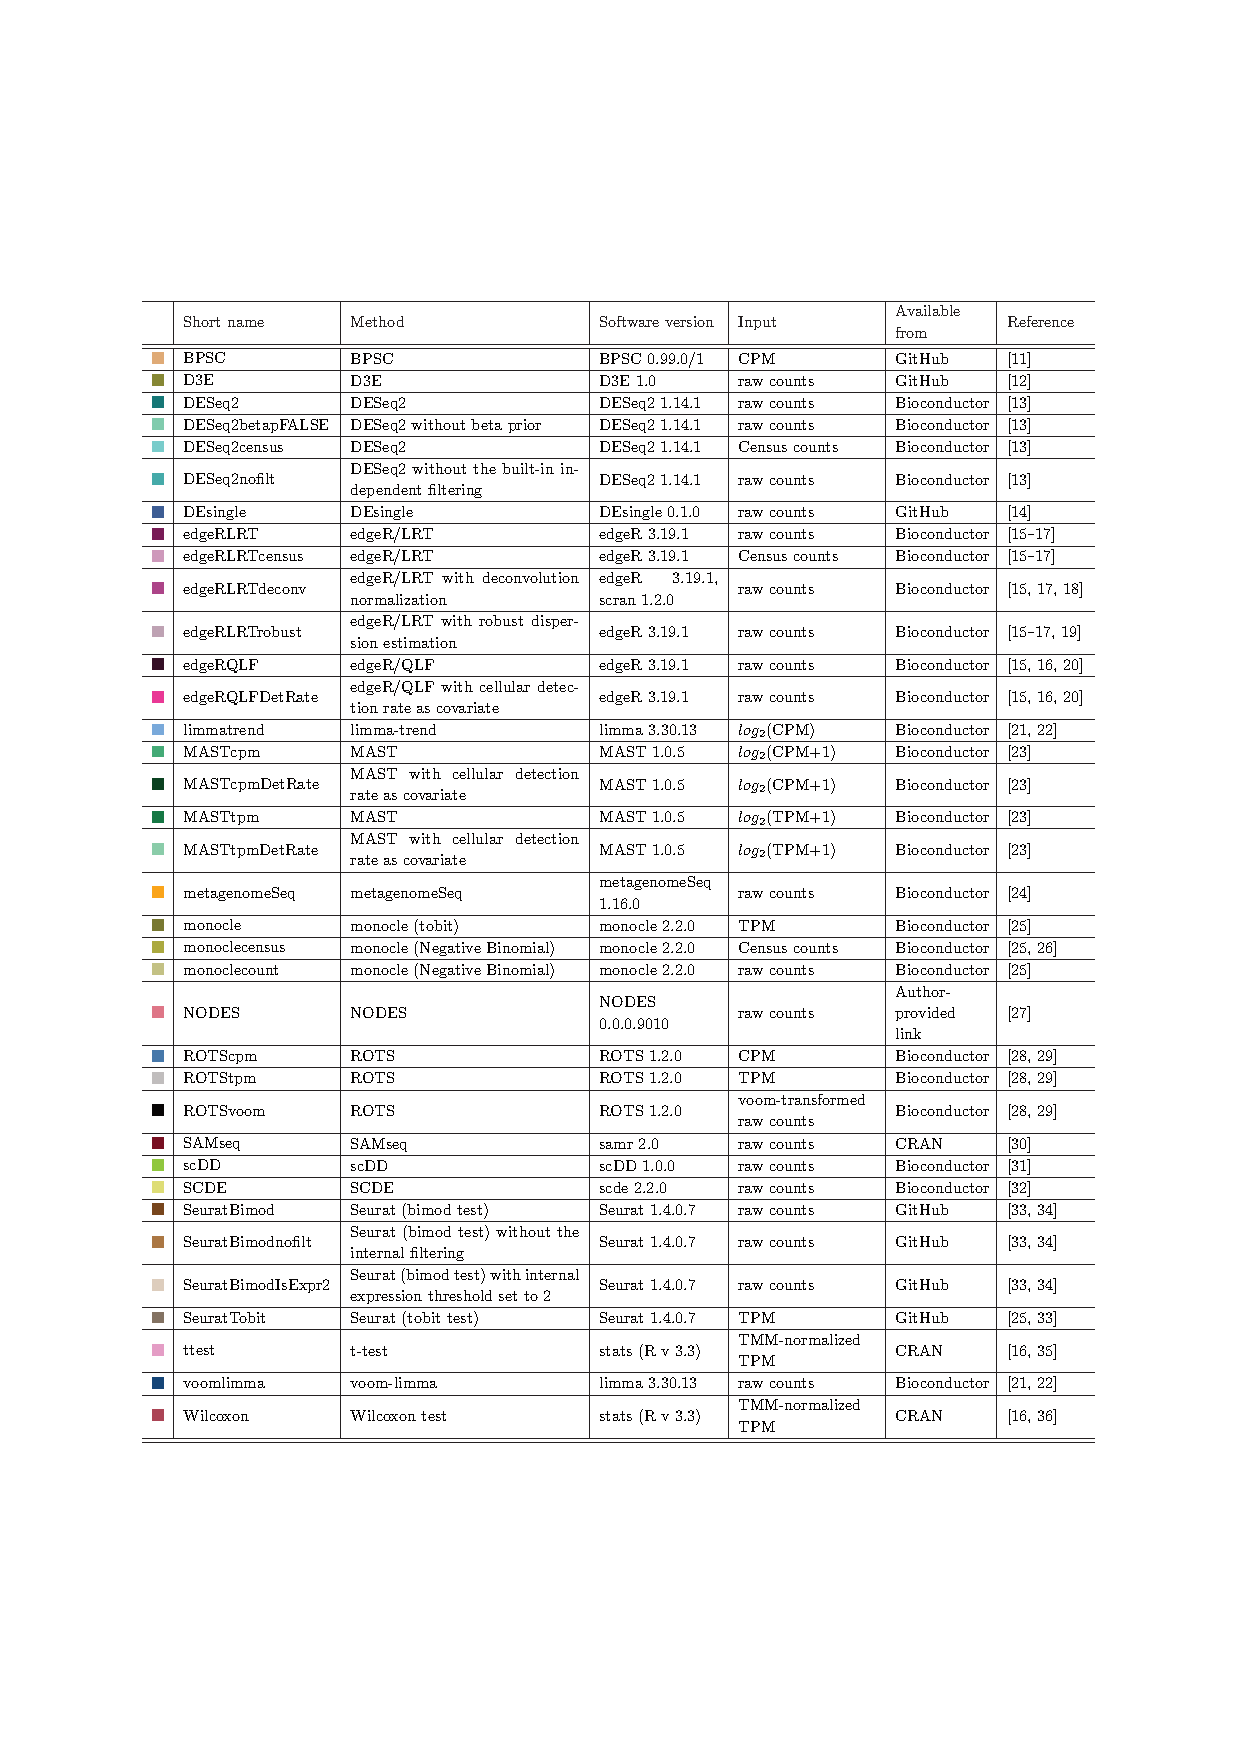
\includegraphics[trim={0 5cm 0 5cm}, clip, width=\paperwidth]{Images/Robinson-2018.pdf}}%
\begin{frame}

\begin{figure}
 \centering
   \begin{tikzpicture}[overlay]
     %\node at (0,0) {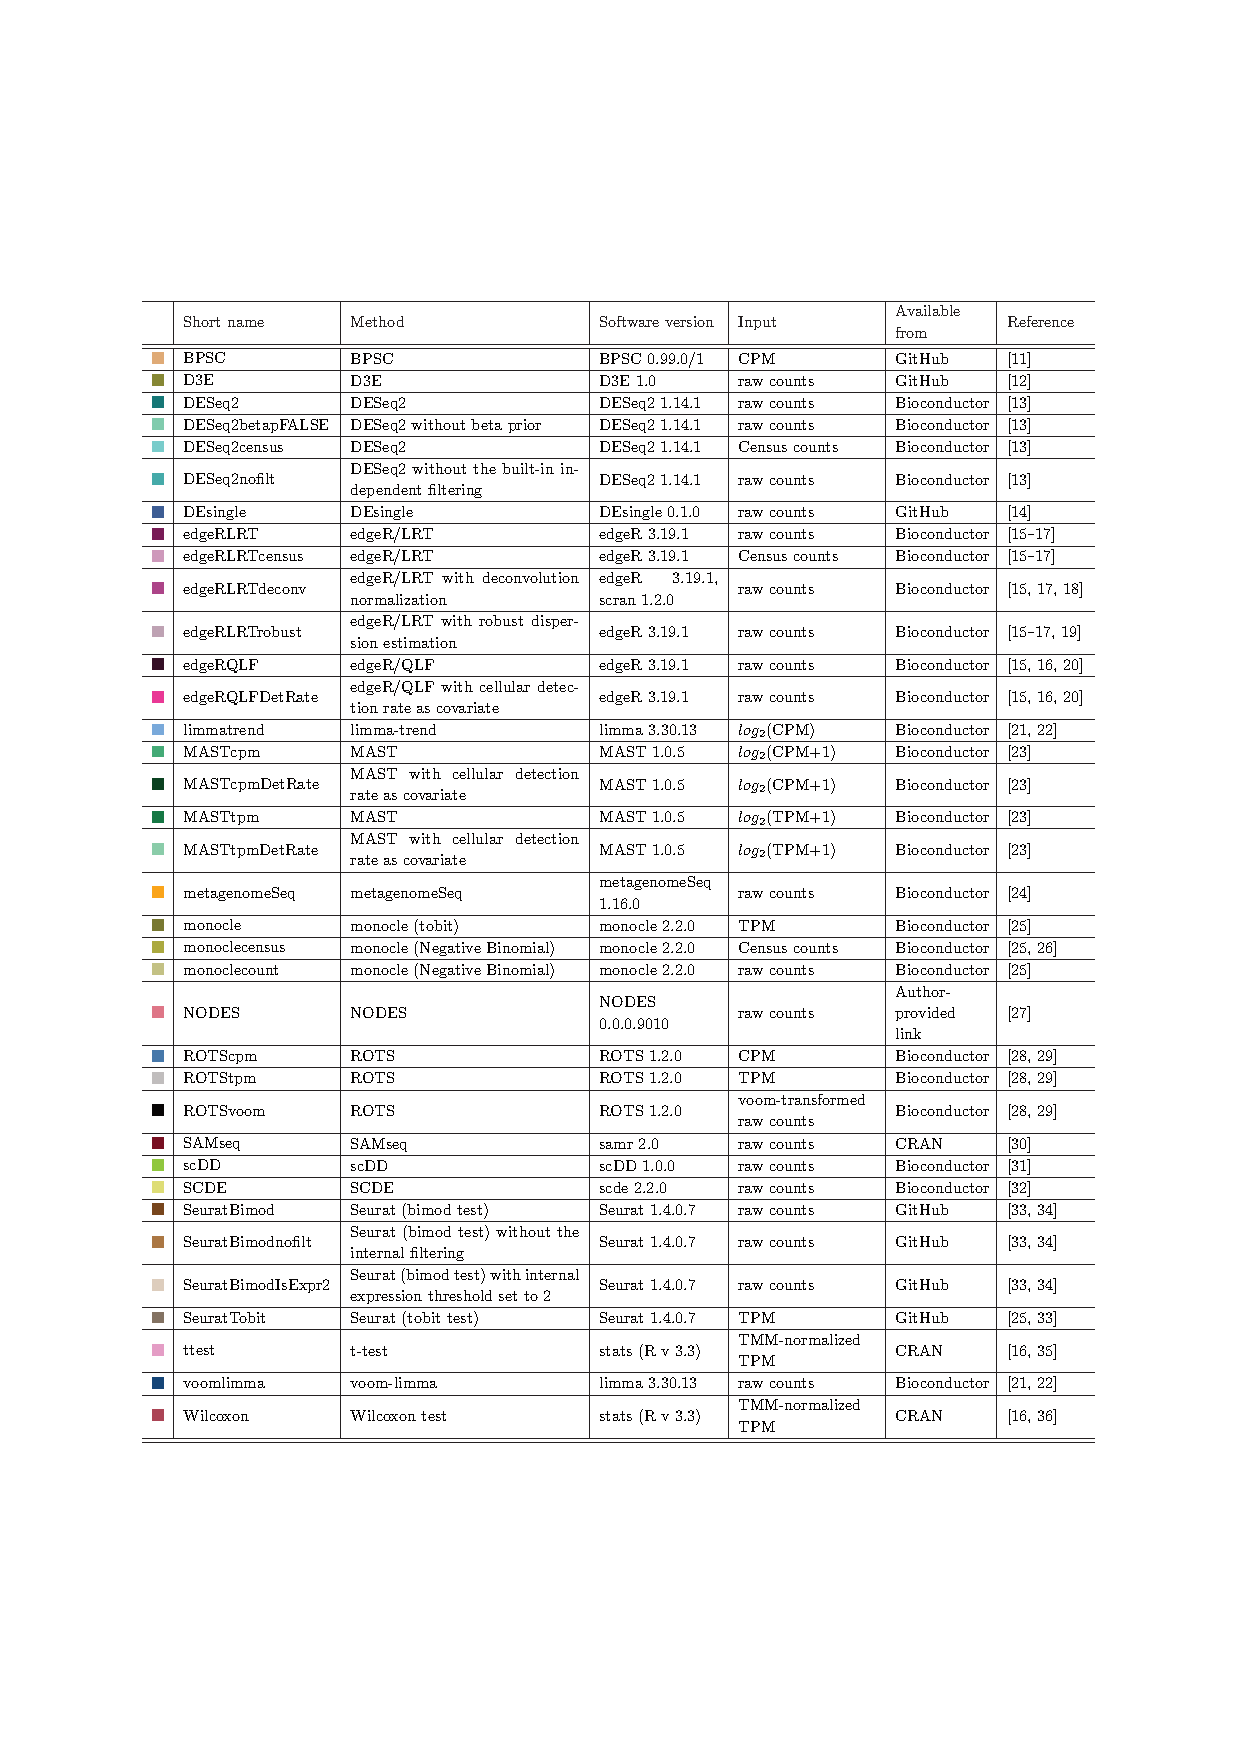
\includegraphics[trim={0 5cm 0 5cm}, clip, height=7.5cm]{Images/Robinson-2018.pdf}};
     \node at (0, -1) {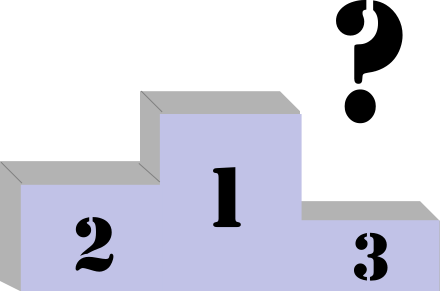
\includegraphics[scale=0.5]{Images/podium.png}};
  \end{tikzpicture}
%\caption{Using Tikz Overlay}
%\insertsection
\end{figure}
\end{frame}
}

\begin{frame}
No ground truth, i.e. no independently validated truth is available for testing \pause
\vspace{0.5cm}
\begin{columns}
\column{0.4\textwidth}
\scriptsize
\begin{block}{Known data}
using data we know something about to get "positive controls"
\end{block} \pause

\begin{block}{Simulated data} 
null-data sets by re-sampling, modeling data sets based on various distributions
\end{block} \pause

\column{0.4\textwidth}
\scriptsize
\begin{block}{Comparing between methods and scenarios}
Comparing numbers of DEs incl. as a function of group size 
\end{block} \pause

\begin{block}{Investigating results}
How does the expression and distributions of detected DEs look like?
\end{block}

\end{columns}
\end{frame}

% % P: Dal Molin
% \begin{frame}
% \frametitle{Learn from methodological papers and/or past studies}
% e.g. \href{https://www.frontiersin.org/articles/10.3389/fgene.2017.00062/full(}{Dal Molin, Barruzo and Di Camilillo, frontiers in Genetics 2017, Single-Cell RNA-Sequencing: Assessment of Differential Expression Analysis Methods}
% \begin{itemize}
% \item 10,000 genes simulated for 2 conditions with sample size of 100 cells each
% \item 8,000 genes were simulated as not differentially expressed using the same distribution (unimodal: NB and bimodal: two-component NB mixture)
% \item 2,000 genes were simulated as differentially expressed according to four types of differential expressions 
% \item real dataset: 44 mouse Embryonic Stem Cells and 44 Embryonic Fibroblsts for positive control
% \item real dataset: 80 single cells as negative control
% \end{itemize}
% \end{frame}


% P: Dal Molin plots
\begin{frame}
False positives (type I error) vs.  false negatives (type II error) \newline
\scriptsize
\href{https://en.wikipedia.org/wiki/Sensitivity_and_specificity}{Sensitivity and specificity} \newline
\href{https://en.wikipedia.org/wiki/Precision_and_recall}{Precision and recall}

\begin{columns}
\column{0.4\textwidth}
\begin{center}
\begin{figure}
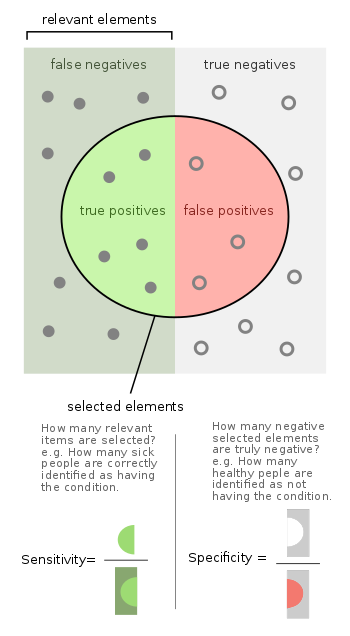
\includegraphics[height=7cm]{Images/sensitivity-specificity}
\end{figure}
\end{center}
\column{0.4\textwidth}
\begin{center}
\begin{figure}
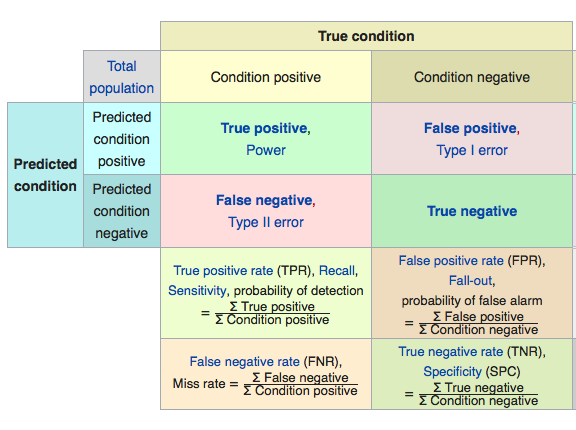
\includegraphics[width=5cm]{Images/confusion-matrix}
\caption{adapted from Wikipedia}
\end{figure}
\end{center}
\end{columns}
\end{frame}


% P: Dal Molin plots
\begin{frame}
False positives (type I error) vs.  false negatives (type II error) \newline
\scriptsize
\href{https://en.wikipedia.org/wiki/Sensitivity_and_specificity}{Sensitivity and specificity} \newline
\href{https://en.wikipedia.org/wiki/Precision_and_recall}{Precision and recall}
\vspace{0.5cm}
\scriptsize
\begin{center}
\begin{figure}
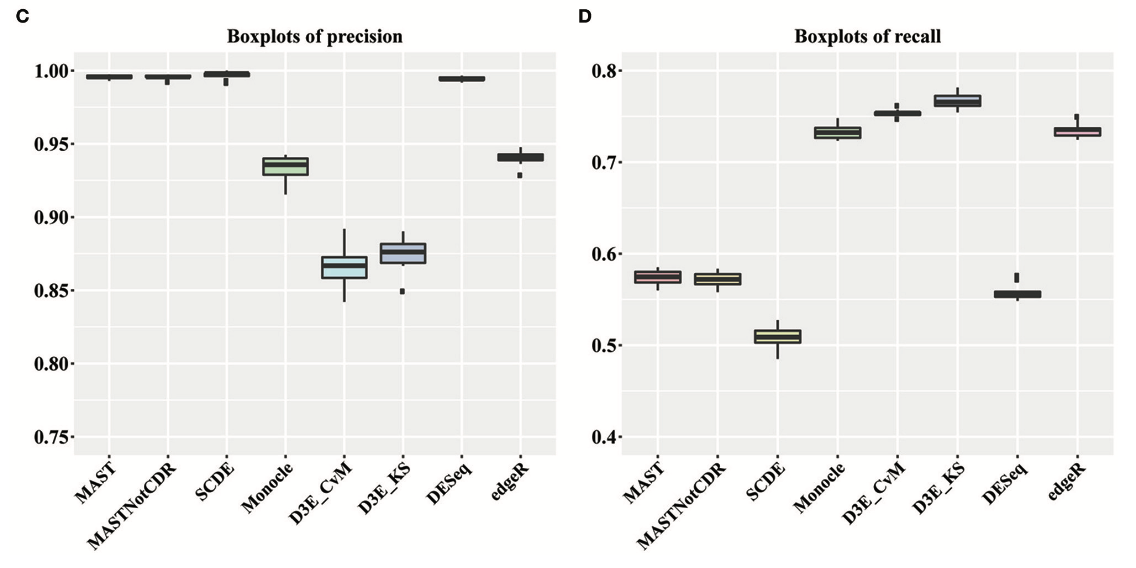
\includegraphics[width=12cm]{Images/DalMolin_fig2cd.png}
\caption{\cite{DalMolin2017}: 2 conditions of 100 cells each simulated with 10 000 genes, out of which 2 000 set to DEs (based on NB and bimodal distributions)}
\end{figure}
\end{center}
\end{frame}


\begin{frame}
%\frametitle{Compare methods}
Consistency
\vspace{0.5cm}
%e.g. \href{Differential expression analyses for single-cell RNA-Seq: old questions on n???}{Miao and Zhang, Quantitative Biology 2016,4: Differential expression analyses for single-cell RNA-Seq: old questions on new data}
\begin{center}
\begin{figure}
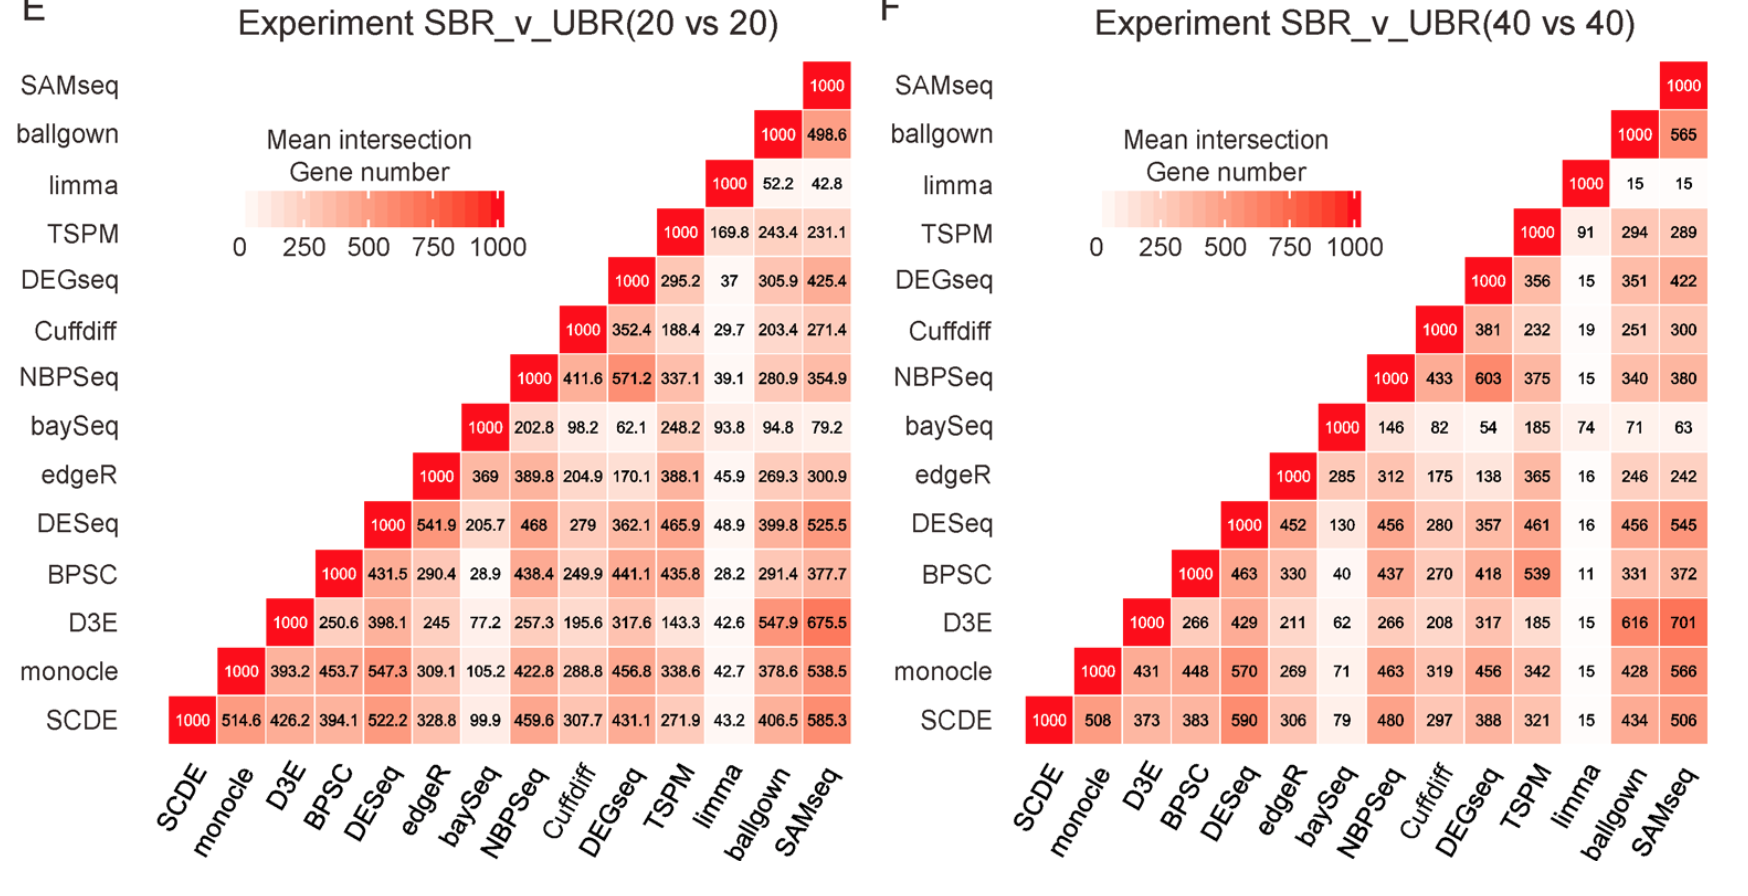
\includegraphics[width=11cm]{Images/Miao_fig1ef.png}
\caption{\cite{Miao2017}}
\end{figure}
\end{center}
\end{frame}

\begin{frame}
And so much more...
\vspace{0.1cm}
\begin{columns}
\column{0.5\textwidth}
\begin{center}
\begin{figure}
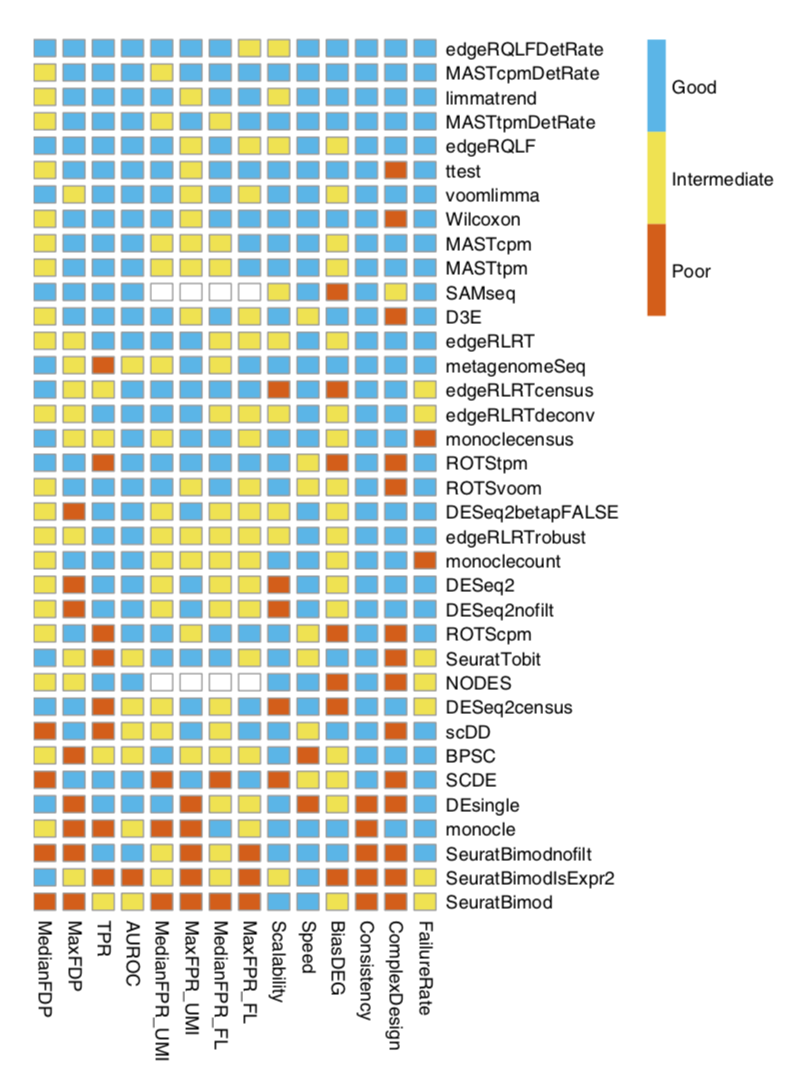
\includegraphics[width=5cm, height=6cm]{Images/Robinson-2018-heatmap}
\caption{\cite{Soneson2018}}
\end{figure}
\end{center}
\column{0.5\textwidth}
\scriptsize
Bias, robustness and scalability in single-cell differential expression analysis
\begin{itemize}
  \item 36 statistical approaches for DE analysis to compare the expression levels in the two groups of cells
  \item based on 9 data sets, with 11 - 21 separate instances (sample size effect)
  \item extensive evaluation metrics incl. number of genes found, characteristics of the false positive detections, robustness of methods, similarities between methods etc. 
  \item \textit{conquer}, a collection of consistently processed, analysis-ready public scRNA-seq data sets
\end{itemize}
\column{0.4\textwidth}
\end{columns}
\end{frame}


\section{Practicalities}
\begin{frame}
\begin{center}
\insertsection
\end{center}
\end{frame}

% P: assess data and distributions
\begin{frame}
\begin{block}{Getting to know your data}
\scriptsize
Example data: 46,078 genes x 96 cells \newline
22,229 genes with no expression at all

\begin{knitrout}
\definecolor{shadecolor}{rgb}{0.969, 0.969, 0.969}\color{fgcolor}
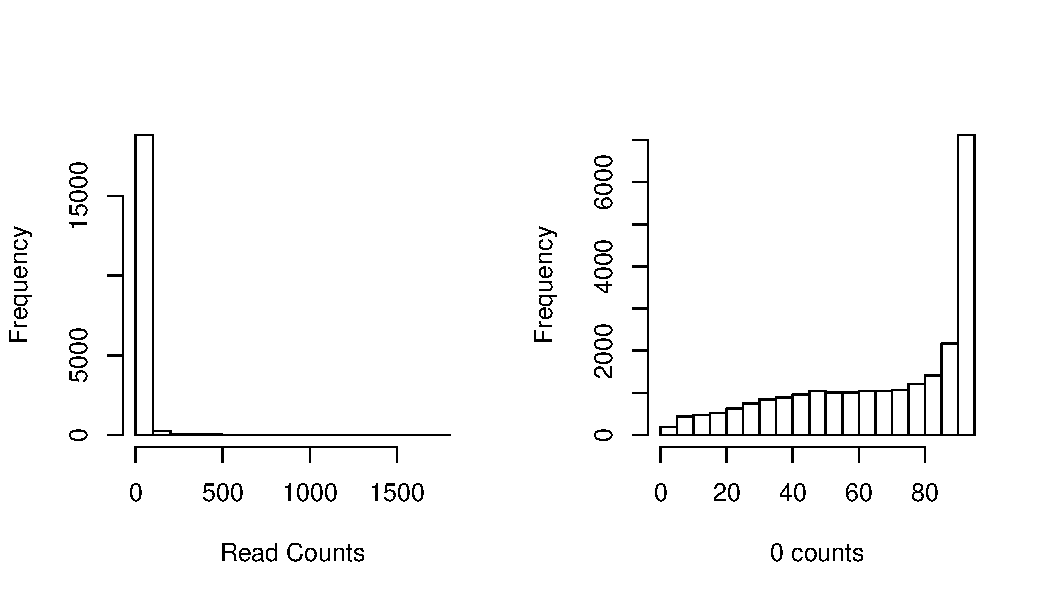
\includegraphics[width=\maxwidth]{figure/knowdata-1} 

\end{knitrout}
\end{block}
\end{frame}


\begin{frame}
\begin{block}{Choosing DE methods}
\vspace{0.7cm}
\begin{center}
\begin{figure}
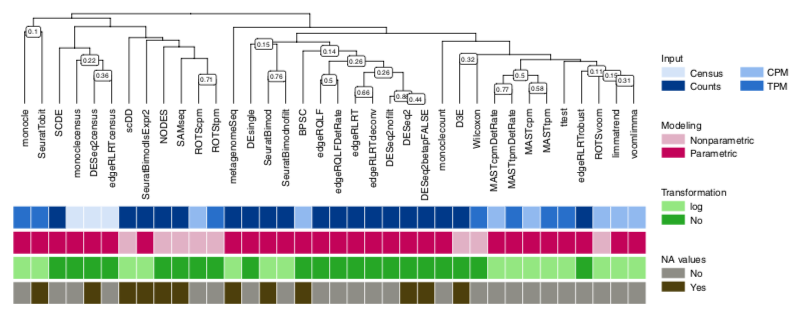
\includegraphics[width=11cm]{Images/Robinson-2018-hcl}
\caption{\cite{Soneson2018}}
\end{figure}
\end{center}
\end{block}
\end{frame}

% P: Rembering the bigger picture
\begin{frame}
\begin{block}{Rembering the bigger picture}

\begin{columns}
\column{0.6\textwidth}
\begin{center}
\begin{figure}
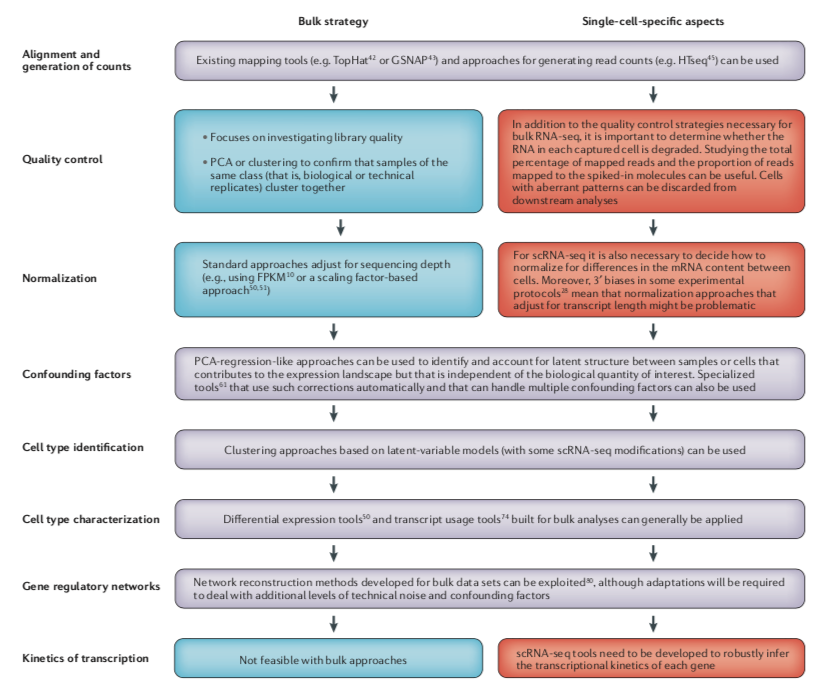
\includegraphics[height=6cm]{Images/Stegle-2015-workflow}
\caption{\cite{Stegle2015}}
\end{figure}
\end{center}

\column{0.4\textwidth}

%\begin{itemize}
\scriptsize
QC filtering \newline \newline
Cell-cycle phase \newline \newline
Normalization of cell-specific biases \newline \newline
Confounding factors, incl. batch effects \newline \newline
Detection rate, i.e the fraction of detected genes per cell \newline \newline
Imputations strategies for dropout values  \newline \newline \newline
What is pragmatic: programming language, platform, speed, collaborative workflows etc.
%\end{itemize}
\end{columns}
\end{block}
\end{frame}

% P: Stay critical
\begin{frame}
\begin{block}{Staying critical}
\begin{center}
\begin{figure}
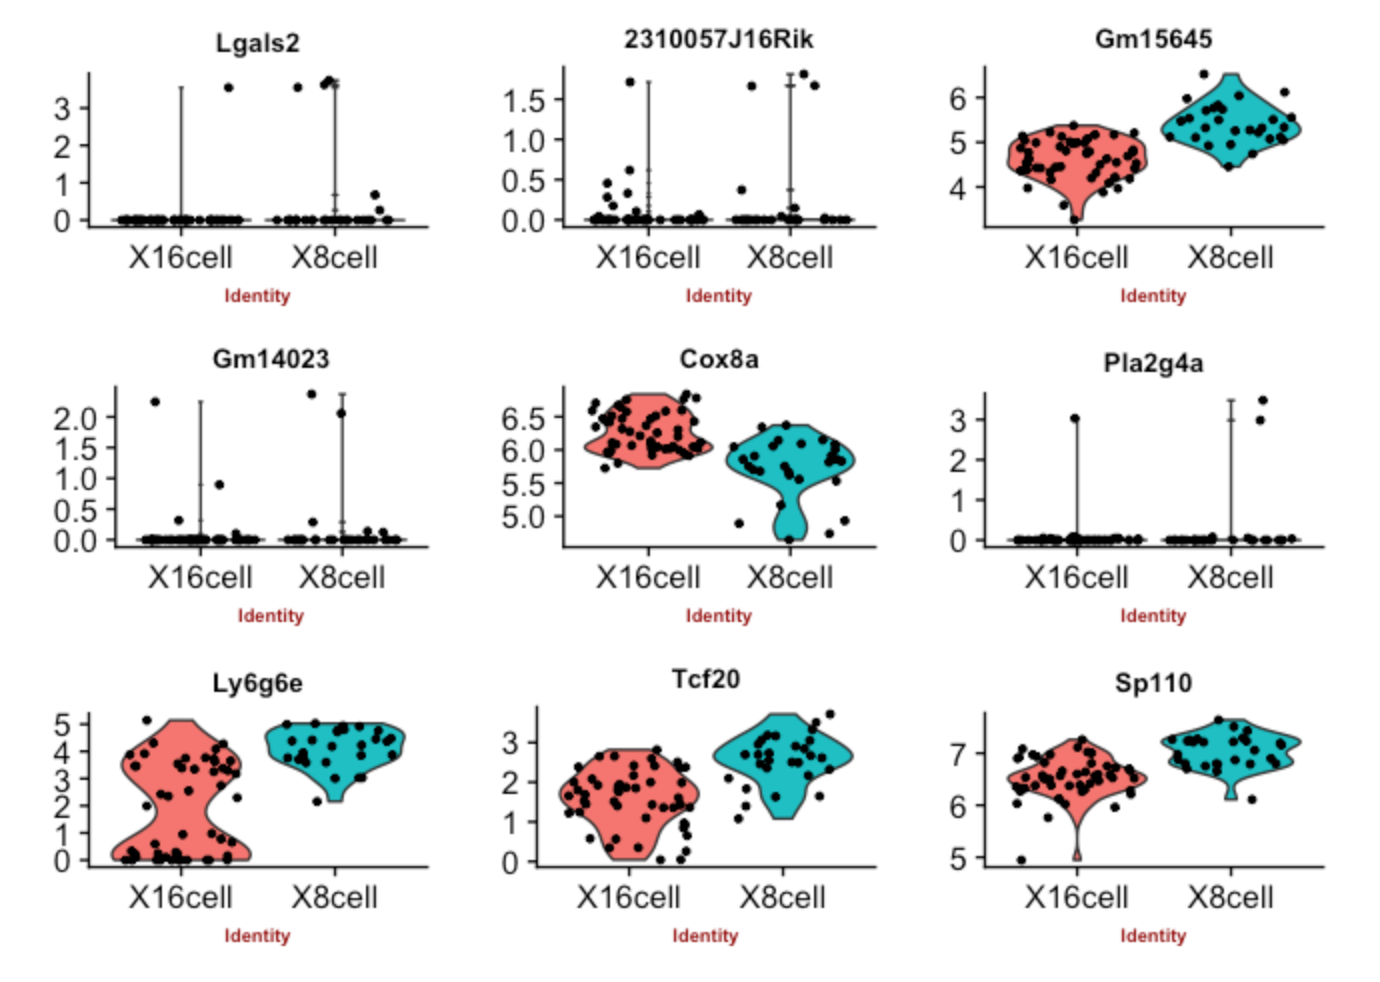
\includegraphics[width=11cm]{Images/asa1.png}
%\caption{based on tutorial examples}
\end{figure}
\end{center}
\end{block}
\end{frame}

% Summary section
\section{Summary}
% \begin{frame}
% \begin{center}
% \insertsection
% \end{center}
% \end{frame}

% Summary: question
\begin{frame}
\begin{center}
\colorbox{blue!10}{What to remember from this hour?}
%\vspace{0.2cm}
\end{center}
\begin{center}
\href{https://www.menti.com}{https://www.menti.com} \& 25 06 78%\pause
\end{center}
\end{frame}

\begin{frame}
\begin{block}{Growing field}
\vspace{0.5cm}
\begin{center}
\begin{figure}
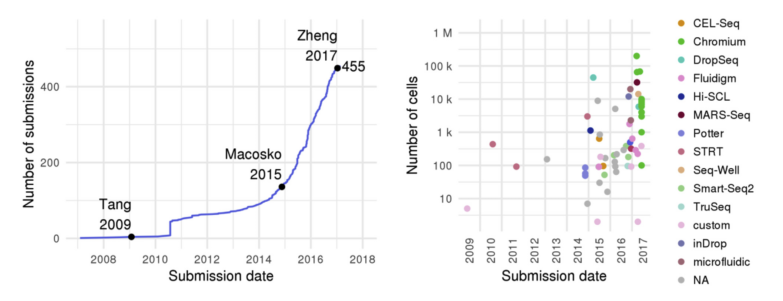
\includegraphics[width=11cm]{Images/Angerer-datasets.png}
\caption{\cite{Angerer2017}}
\end{figure}
\end{center}
% \begin{center}
% \begin{figure}
% 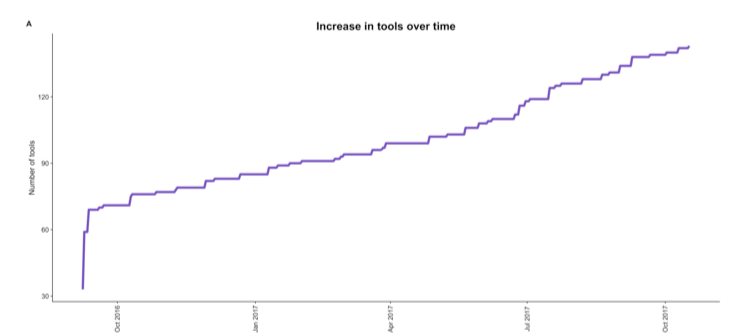
\includegraphics[height=3cm]{Images/Oshlack-tools.png}
% \caption{\cite{Zappia2018}}
% \end{figure}
% \end{center}
\end{block}
\end{frame}

\begin{frame}
\begin{block}{Growing field}
\href{https://www.scrna-tools.org/tools}{https://www.scrna-tools.org/tools}
\vspace{0.5cm}
\begin{center}
\begin{figure}
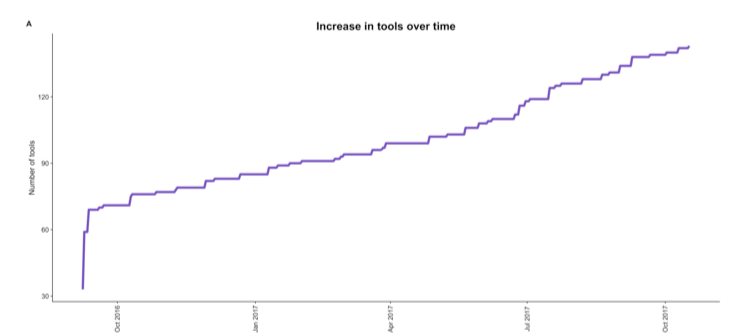
\includegraphics[height=5cm]{Images/Oshlack-tools.png}
\caption{\cite{Zappia2018}}
\end{figure}
\end{center}
\end{block}
\end{frame}

% Summary points
\begin{frame}
\begin{block}{Summary}
\begin{itemize}
\scriptsize
\item scRNA-seq is a rapidly growing field
\item DE is a common task so many newer and better methods will be developed
\item understanding basic statistical concepts enables one to think more like a statistician: to choose and evaluate methods given data set
\item staying critical, staying updated, staying connected
\end{itemize}
\end{block}
\end{frame}

% % Tutorial
% \section{DE tutorial}
% \begin{frame}
% \begin{center}
% \insertsection
% \end{center}
% \end{frame}

% % Tutorial points
% \begin{frame}
% \begin{block}{DE tutorial}
% Based on the dataset used is single-cell RNA-seq data (SmartSeq) from mouse embryonic development from Deng. et al. Science 2014, Vol. 343 no. 6167 pp. 193-196, "Single-Cell RNA-Seq Reveals Dynamic, Random Monoallelic Gene Expression in Mammalian Cells".
% \begin{itemize}
% \item check for differentially expressed genes between 8-cell and 16-cell stage embryos
% \item with many methods incl. SCDE, MAST, SC3 package, Pagoda, Seurat
% \item and compare the results, trying to decide on the best DE method for the dataset
% \end{itemize}
% \end{block}
% \end{frame}

% \section{Finally}
% \begin{frame}
% \begin{center}
% Thank you for attention
% \newline
% \newline
% Questions?
% \newline
% \newline
% Enjoy the rest of the course
% \newline
% \newline
% olga.dethlefsen@nbis.se
% \end{center}
% \end{frame}

\section{Bibliography}
\begin{frame}
\printbibliography
%\bibliography{scRNA}
\end{frame}


% % P: Dal Molin
% \begin{frame}
% \frametitle{Learn from methodological papers and/or past studies}
% e.g. \href{https://www.frontiersin.org/articles/10.3389/fgene.2017.00062/full(}{Dal Molin, Barruzo and Di Camilillo, frontiers in Genetics 2017, Single-Cell RNA-Sequencing: Assessment of Differential Expression Analysis Methods}
% \begin{itemize}
% \item 10,000 genes simulated for 2 conditions with sample size of 100 cells each
% \item 8,000 genes were simulated as not differentially expressed using the same distribution (unimodal: NB and bimodal: two-component NB mixture)
% \item 2,000 genes were simulated as differentially expressed according to four types of differential expressions 
% \item real dataset: 44 mouse Embryonic Stem Cells and 44 Embryonic Fibroblsts for positive control
% \item real dataset: 80 single cells as negative control
% \end{itemize}
% \end{frame}

\end{document}
